Recap: statistical analysis with linear models. Selecting the right model is a key challenge. Ideally, data collection and model building go hand in hand. We can analyse \begriff{observational data} (data observed in natural setting) or \begriff{experimental data} (we control the explanatory variables). The former finds correlations, the latter can establish causal links. 

\subsection{Designing an experiment}

\begin{proposition}
	The study of experimental design originated with \person{R. A. Fischer}'s work in the UK in the 1900s.
\end{proposition}

In an experiment, we collect data in a structured way. We decide on:
\begin{itemize}
	\item what to measure - \textbf{response}
	\item what to measure the response on - \textbf{experimental unit}
	\item the independent variables whose effect we study - \textbf{factors}
	\item the combinations of factors we want to study - \textbf{treatments}
	\item how many data points to collect  - \textbf{sample size}
	\item how to assign treatments to experimental units 
\end{itemize}

\begin{example}
	Compare the range of three electric car models. Range is the response, car model is a factor with three levels. With only one factor, there are no further treatments. Experimental units are cars and we can decide how many of each model we want to test.
\end{example}

The more data we collect, the more certain we can be about trends we find. However, collecting data is often expensive. Measurement errors, environmental variation or other effects lead to \begriff{noise} in data. Noise-reducing experimental design can be used to counter this. Once we have identified factors we want to investigate, we have to think carefully about which treatment to test, to get the most out of our experiment (volume-increasing design).

\subsubsection{Noise-reducing design}

Noise-reducing designs assign treatments to experimental units in such a way that extraneous noise is reduced. The simplest approach: \begriff{completely randomised design} - treatments assigned randomly to experimental units.

\begin{example}
	Length of time to assemble a watch using three different methods A, B and C. Select 15 workers and assign them randomly to A, B or C.
	
	But: assembly times could vary substantially between workers. This could skew our findings. To avoid this, we could get 5 workers to each use A, B or C in turn (randomised block design).
\end{example}

In \begriff{randomised block design}, we compare $p$ treatments by $b$ blocks. Each block contains $p$ relatively homogeneous (or identical) experimental units. The $p$ treatments are assigned randomly to experimental units in each block (one experimental unit assigned per treatment).

These experimental designs can be captured in linear models to investigate differences in the mean response across treatments. For the watch example:
\begin{itemize}
	\item Mode for completely randomised design: $Y_i = \beta_0 + \beta_1x_{1i} + \beta_2x_{2i} + \epsilon_i$,
	\begin{align}
		x_{1i} &= \begin{cases}
		1 & \text{if worker $i$ uses method A} \\ 0 & \text{if not}
		\end{cases} \notag \\
		x_{2i} &= \begin{cases}
		1 & \text{if worker $i$ uses method B} \\ 0 & \text{if not}
		\end{cases} \notag
	\end{align}
	... selected method C as the base level.
	\item Model for randomised block design:
	\begin{align}
		Y_ i = \beta_0 + \underbrace{\beta_1x_{1i} + \beta_2x_{2i}}_{\text{treatment effects}} + \underbrace{\beta_3x_{3i} + \beta_4x_{4i} + \beta_5x_{5i} + \beta_6x_{6i}}_{\text{block effects}} + \epsilon_i \notag
	\end{align}
	... $x_{3i}$ up to $x_{6i}$ are dummy variables for which worker assembles.
\end{itemize}

We can use the usual methods to test hypothesis on our data (e.g. t-test for individual parameters, F-test, Likelihood-ratio test for nested models).

\subsubsection{Volume-increasing design}

Volume-increasing designs combine factors in experiments into treatments that are maximally informative.

\begin{example}
	An electricity company wants to measure customer satisfaction for two levels of peak time price increase, $x_1$, and two different peak period lengths, $x_2$ (2 levels). How should the levels of factors $x_1$ and $x_2$ be combined into treatments?
	\begin{itemize}
		\item Option 1: keep one factor fixed and vary the other. This is consistent with block designs. However, it misses interactions between factors.
		\item Option 2: consider all possible combinations of factor levels (\begriff{complete factorial design}). For this example, we call it a $2\times 2$ factorial design.
	\end{itemize}
\end{example}

\textbf{Warning:} if many factors are tested, complete factorial designs require a lot of treatments.

Complete factorial designs can be captured in linear models with interaction terms. For this example the model is
\begin{align}
	Y_i = \beta_0 + \underbrace{\beta_1x_{1i} + \beta_2x_{2i}}_{\text{main effects}} + \underbrace{\beta_3x_{1i}x_{2i}}_{\text{interaction}} + \epsilon_i \notag
\end{align}
... $x_{1i}$ and $x_{2i}$ are dummy variables for peak time price increase levels and peak period length levels, respectively. The number of parameters is the same as the number of treatments. This is always the case for complete factorial designs. Thus, we need replicate measurements for each treatment.

Aside: this also works for quantitative predictors.

\subsection{Selecting the sample size}

Deciding how many data points to collect is important: On the one hand, the more data we have, the more certain we can be about observed trends (e.g. standard errors for parameter estimates in lecture 6). On the other hand, collecting data is expensive, so we only want to collect what's necessary.

Power analysis allows us to determine the sample size required to detect an effect of a given size with a given degree of confidence. In general, the smaller the effect and the more confident we want to be, the more replicates we need.

\subsection{Introduction to ANOVA}

Analysis of variance (ANOVA) is a statistical analysis for comparing means in experiments across different treatments. ANOVA is equivalent to analysing linear models. Before computers, ANOVA simplified calculations and it's still commonly used and referred to. 

Intuition for ANOVA: consider the variation within and between treatments.
\begin{center}
	\begin{tikzpicture}[scale=0.9]
		\begin{axis}[
			xmin=0.5, xmax=2.5, xlabel=treatment,
			ymin=3, ymax=9, ylabel=some measure (some unit),
			axis x line=bottom,
			axis y line=left,
		]
		\addplot[blue, only marks, mark=x] coordinates {
			(1.00,5.27)
			(1.00,5.92)
			(1.00,3.87)
			(1.00,5.43)
			(1.00,5.16)
		};
		\draw[cyan] (axis cs: 0.5,5) -- (axis cs: 1.5,5);
		\addplot[red, only marks, mark=x] coordinates {
			(2.00,6.73)
			(2.00,7.61)
			(2.00,7.15)
			(2.00,6.99)
			(2.00,7.14)
		};
		\draw[orange] (axis cs: 1.5,7) -- (axis cs: 2.5,7);
		\end{axis}
	\end{tikzpicture}
	\begin{tikzpicture}[scale=0.9]
	\begin{axis}[
	xmin=0.5, xmax=2.5, xlabel=treatment,
	ymin=3, ymax=9, ylabel=some measure (some unit),
	axis x line=bottom,
	axis y line=left,
	]
	\addplot[blue, only marks, mark=x] coordinates {
		(1.00,6.01)
		(1.00,3.19)
		(1.00,6.08)
		(1.00,7.45)
		(1.00,5.73)
	};
	\draw[cyan] (axis cs: 0.5,5) -- (axis cs: 1.5,5);
	\addplot[red, only marks, mark=x] coordinates {
		(2.00,8.03)
		(2.00,7.73)
		(2.00,6.70)
		(2.00,7.29)
		(2.00,6.21)
	};
	\draw[orange] (axis cs: 1.5,7) -- (axis cs: 2.5,7);
	\end{axis}
	\end{tikzpicture}
\end{center}

In ANOVA, we consider
\begin{align}
	F = \frac{\text{between-treatment variation}}{\text{within-treatment variation}} \notag
\end{align}

\subsubsection{One-way ANOVA}

Consider a one-factor completely randomised design, i.e. a number pf $p$ factor levels and experimental units assigned randomly to them. We have seen that this can be modelled as
\begin{align}
	Y_i = \beta_0 + \beta_1x_{1i} + \dots + \beta_{p-1}x_{p-1,i} + \epsilon_i \notag
\end{align}
where the $x_{ji}$s are dummy variables for the factor levels. We wish to compare the means to response, $\mu_j$, across treatments $j$ and test the null hypothesis $H_0$: $\mu_1 = \mu_2 = \dots = \mu_p$. Suppose the model above, treatment 1 is the base level, them $\beta_0 = \mu_1$, $\beta_1 = \mu_2 - \mu_1$, ..., $\beta_{p-1} = \mu_p - \mu_1$. So the $H_0$ above is equivalent to $H_0$: $\beta_1 = \beta_2 = \dots = \beta_{p-1} = 0$. This is one-way ANOVA. It is the same as an F-test on the corresponding linear model. It shows that at least two treatment means differ. The F-statistic is computed from sums of squared errors (no model fitting required).

\begin{example}
	A study on the strength of different structural beams (\person{Hogg}, 1987). The MATLAB command is \texttt{anova1}.
	
	\begin{center}
		\begin{tikzpicture}
		\begin{axis}[
		xmin=0.5, xmax=3.5,
		ymin=74, ymax=87,
		boxplot/draw direction=y,
		axis x line = bottom,
		axis y line = left,
		xtick={1,2,3},
		xticklabels={steel, alloy1, alloy2},
		ylabel=deflection under load (1/1000 in),
		xlabel=type of beam
		]
		\addplot+ [boxplot prepared={
			lower whisker=79, 
			lower quartile=82.5,
			median=84.5, 
			upper quartile=86,
			upper whisker=87},
		] coordinates {};
		\addplot+ [boxplot prepared={
			lower whisker=74, 
			lower quartile=75,
			median=76.5, 
			upper quartile=78,
			upper whisker=82},
		] coordinates {};
		\addplot+ [boxplot prepared={
			lower whisker=82, 
			lower quartile=78,
			median=79, 
			upper quartile=79,
			upper whisker=77},
		] coordinates {};
		\end{axis}
		\end{tikzpicture}
	\end{center}
	\begin{center}
		\begin{tabular}{c|c|c|c|c|c}
			\textbf{Source} & \textbf{SS} & \textbf{degrees of freedom} & \textbf{MS} & \textbf{F} & \textbf{Prob} $>$ \textbf{F} \\
			\hline
			Groups & 184.8 & 2 & 92.4 & 15.4 & 0.0002 \\
			Error & 102 & 17 & 6 & & \\
			Total & 286.8 & 19 & &
		\end{tabular}
	\end{center}
	
	... this suggests that at least two beams differ in strength.
\end{example}

\subsubsection{Two-way ANOVA}

Consider a complete factorial design with two factors, one of which has three and the other has two levels. We have seen that this can be modelled as:
\begin{align}
	Y_i = \beta_0 + \beta_1x_{1i} + \beta_2x_{2i} + \beta_3w_{1i} + \beta_4x_{1i}w_{1i} + \beta_5x_{2i}w_{1i} + \epsilon_i \notag
\end{align}
where $x_{1i}$ and $x_{2i}$ are dummy variables for the first factor and $w_{1i}$ is a dummy variable for the second factor. Analogously to the one-way ANOVA, in two-way ANOVA, we perform a number of F-tests to compare the mean of the response across treatments. E.g. to test for interactions, we test $H_0$: $\beta_4 = \beta_5 = 0$. Testing if the mean response for levels of the first factor are equal, requires $H_0$: $\beta_1 = \beta_2 = 0$. Essentially, we use F-tests to compare nested models. These tests on multiple parameters simultaneously (e.g. if factors have more than 2 levels). They can show that at least two treatment means differ.

\begin{center}
	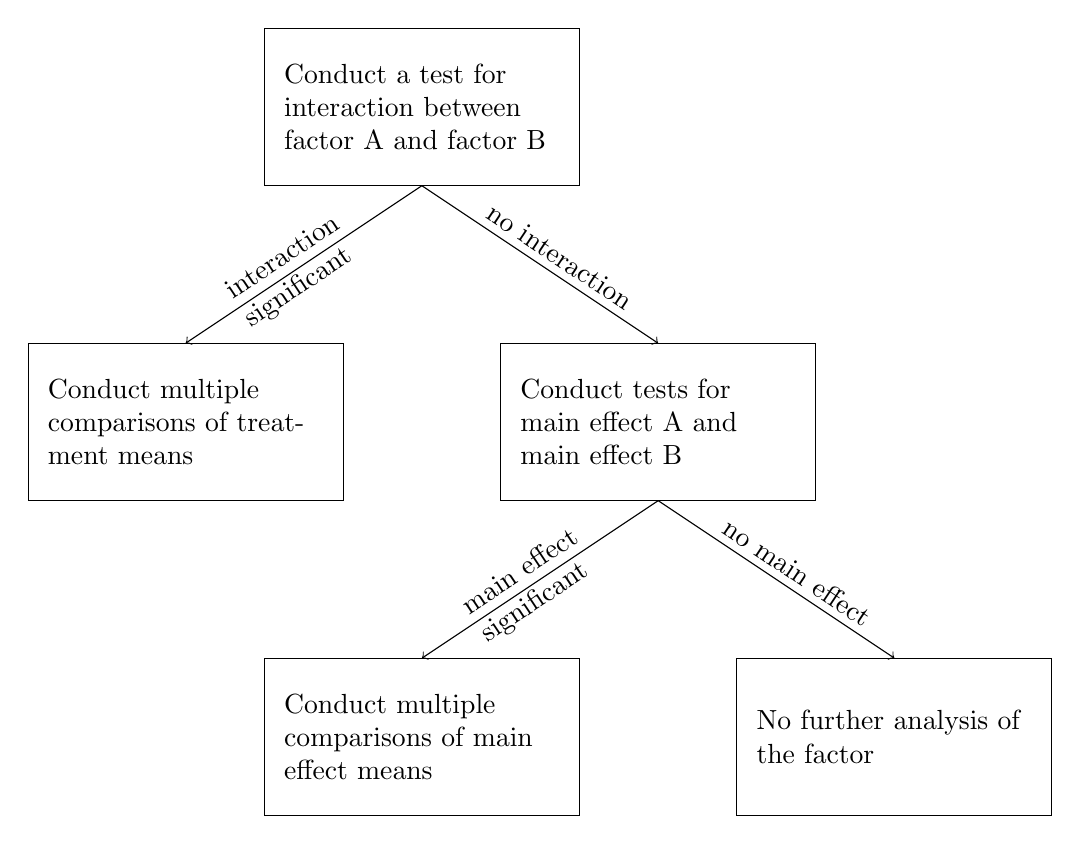
\begin{tikzpicture}
	\draw (-2,0) rectangle (2,2) node[text width=3.5cm,pos=.5] {Conduct a test for interaction between factor A and factor B};
	\draw (-5,-4) rectangle (-1,-2) node[text width=3.5cm,pos=.5] {Conduct multiple comparisons of treatment means};
	\draw (1,-4) rectangle (5,-2) node[text width=3.5cm,pos=.5] {Conduct tests for main effect A and main effect B};
	\draw (-2,-8) rectangle (2,-6) node[text width=3.5cm,pos=.5] {Conduct multiple comparisons of main effect means};
	\draw (4,-8) rectangle (8,-6) node[text width=3.5cm,pos=.5] {No further analysis of the factor};
	
	\draw[->] (0,0) -- (-3,-2);
	\node[text width=2cm,rotate=33.7] at (-1.5,-1) (a) {interaction significant};
	\draw[->] (0,0) -- (3,-2);
	\node[text width=2.5cm,rotate=-33.7] at (1.9,-1) (b) {no interaction};
	\draw[->] (3,-4) -- (0,-6);
	\node[text width=2cm,rotate=33.7] at (1.5,-5) (c) {main effect significant};
	\draw[->] (3,-4) -- (6,-6);
	\node[text width=2.5cm,rotate=-33.7] at (4.9,-5) (d) {no main effect};
	\end{tikzpicture}
\end{center}

Diagram from: \person{W. Mendenhall} and \person{T. Sincich}, \textit{Statistics for Engineering and the Sciences}, CRC Press, 2016.

\subsection{Observational data - sampling}

Sometimes conducting experiments is not possible. Sampling methods are used to collect observational data in a systematic way. 

\begin{example}
	Opinion poll to assess the voting intentions of the population before elections. It's not enough to just ask people in Bristol.
\end{example}

Basic idea: consider a population. Ideally we would like to measure everyone. This is not possible. Sampling is the process of selecting a subset (a \begriff{statistical sample}) of units from the population to estimate whatever we are interested in for the whole population.
\begin{itemize}
	\item \textbf{Probability sampling:} every unit in the population has a probability of being selected and this can be calculated.
	\item \textbf{Nonprobability sampling:} not the product of a randomised selection process.
\end{itemize}

Different sampling methods can be used, depending on information available, costs and accuracy requirements, e.g.
\begin{itemize}
	\item \textbf{Simple random sampling:} all units in the population have the same probability of being selected (if the sample is small, this may not be representative).
	\item \textbf{Systematic sampling:} arrange population in some order, select units at regular intervals. If starting point or order is randomised, this is a probability sampling.
	\item \textbf{Stratified sampling:} organise population according to some categories into separate \begriff{strata} and sample randomly from those.
	\item There are many additional methods, e.g. \textbf{voluntary sampling}, \textbf{accidental sampling}, \textbf{quota sampling},...
\end{itemize}